\section{Arquitectura}
Primero vamos a presentar la arquitectura del core de nuestro sistema (ARS), es decir de la parte que se encarga de realizar todas las operaciones sobre los datos.

\begin{figure}[h]
  \begin{subfigure}{.5\textwidth}
    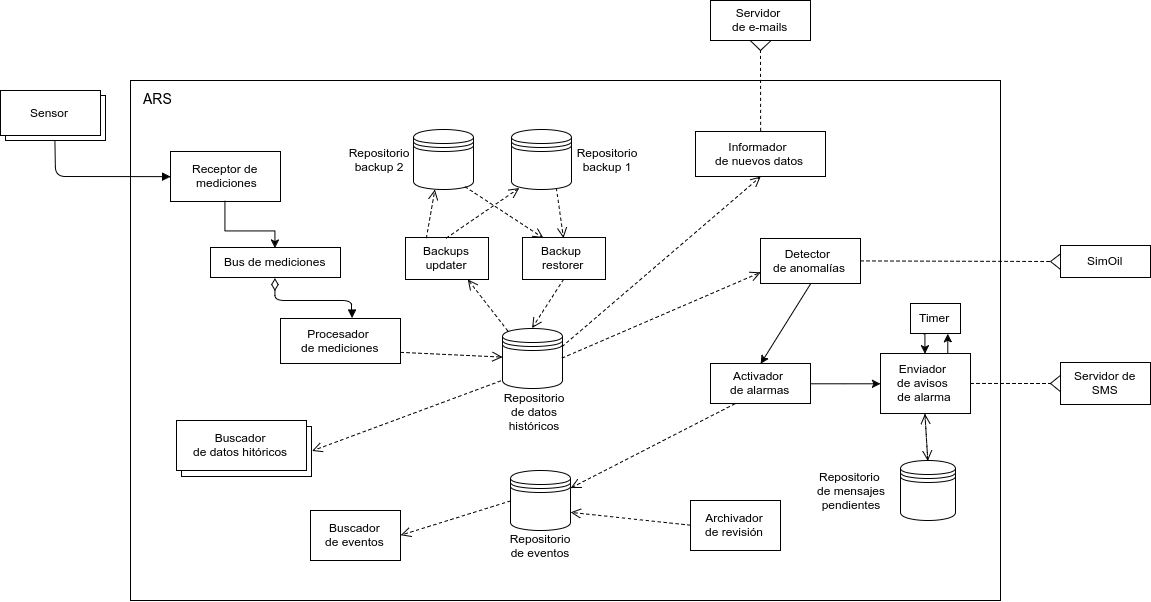
\includegraphics[width=\textwidth]{imagenes/diagramas/core.png}
  \end{subfigure}
  \label{}
  \caption{Diagrama de componentes y conectores del core}
\end{figure}

En la figura se puede observar que poseemos un componente llamado receptor de mediciones el cual, como su nombre lo indica, recibe las mediciones enviadas por los sensores.
Esta es la manera en la que los datos ingresan a ARS. El receptor de mediciones publica en un bus las mediciones para que
el procesador de mediciones las reciba luego. El procesador de mediciones es el encargado de realizar el trabajo de limpieza y agregación de
los datos para terminar colocando los resultados en un repositorio histórico de datos, la arquitectura interna de este componente la explicaremos más adelante.
Mientras tanto hay un componente dedicado a detectar anomalías, el mismo revisa cada cierto período de longitud configurable si hay nuevos datos en el
repositorio de datos históricos. Para detectar las anomalías ejecuta algoritmos de big data y machine learning para lograr su propósito y se llega a encontrar
datos no esperados se lo comunica inmediatamente al activador de alarmas. El activador de alarmas procede a escribir el evento en un repositorio de eventos
y le comunica el evento al enviador de avisos de alarma para que éste último envie el mensaje por una interfaz SMS. Notar que como la
interfaz SMS no siempre está disponible el enviador de avisos de alarma reintenta los envíos cada cierto tiempo.
El informador de nuevos datos es el componente encargado de comunicarle al ente regulador por e-mail que hay nuevos datos en ARS, para lograr su cometido lee el repositorio de
datos históricos. Dado que es crucial para nuestra arquitectura tener un repositorio de datos históricos decidimos darle disponibilidad
mediante la realización de un backup, hay un componente (Backups updater) que realiza el backup en los repositorios de backup 1 y 2, en tanto el otro componente (Backup restorer) actúa en cuanto el repositorio
de datos históricos deja de estar disponible
Los componentes Buscador de datos hitóricos, Buscador de eventos y Archivador de revisión los explicaremos más adelante dado que están relacionados con las interfaces de usuario.
